\documentclass[tikz]{standalone}

\tikzstyle{node}=[draw=#1,fill=#1!20]

\newcommand{\vertex}[6]{\node[shape=circle,fill=black, scale=0.5,label=#1:{#2},label=#5:{\tiny\texttt{\color{blue}#6}},#4] (#3)  {};}
\newcommand{\myedge}[4]{ \draw[->] (#1) edge node[#2] {#3} (#4);}


\begin{document}
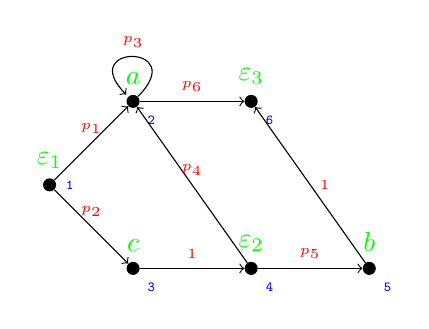
\begin{tikzpicture}[align=center,node distance=3cm]
    % equidistant points and arc
    \vertex{above}{$\color{green}\varepsilon_1$}{s}{}{right}{1}
    \vertex{above}{$\color{green}a$}{b1}{above right of=s}{below right}{2}
    \vertex{above}{$\color{green}c$}{b2}{below right of=s}{below right}{3}
    \vertex{above}{$\color{green}\varepsilon_2$}{e2}{right of=b2}{below right}{4}
    \vertex{above}{$\color{green}b$}{b}{right of=e2}{below right}{5}
    \vertex{above}{$\color{green}\varepsilon_3$}{f}{right of=b1}{below right}{6}
    
    
    \myedge{s}{above}{$\scriptscriptstyle{\color{red}p_1}$}{b1}
    \myedge{s}{above}{$\scriptscriptstyle{\color{red}p_2}$}{b2}
    \myedge{b2}{above}{$\scriptscriptstyle{\color{red}1}$}{e2}
    \myedge{e2}{above}{$\scriptscriptstyle{\color{red}p_4}$}{b1}
    \myedge{e2}{above}{$\scriptscriptstyle{\color{red}p_5}$}{b}
    \myedge{b}{right}{$\scriptscriptstyle{\color{red}1}$}{f}
    \myedge{b1}{above}{$\scriptscriptstyle{\color{red}p_6}$}{f}
    
    \draw[->,shorten >=1pt] (b1) edge [in=135,out=45,loop,looseness=20] node [above] {$\scriptscriptstyle{\color{red}p_3}$} (b1);
\end{tikzpicture}

\end{document}
